\documentclass[11pt]{article}

\usepackage[T1]{fontenc}
\usepackage[margin=1in]{geometry}
\usepackage{times}
\usepackage{url}
\usepackage{hyperref}
\usepackage{graphicx}
\usepackage{array}
\usepackage{tabularx}
\usepackage{booktabs}
\usepackage{enumitem}
\usepackage{amsmath}
\usepackage{tikz}
\usetikzlibrary{arrows.meta, positioning, shapes.geometric, fit, calc}

\hypersetup{
  colorlinks=true,
  linkcolor=blue,
  citecolor=blue,
  urlcolor=blue
}

\setlist[itemize]{leftmargin=*}
\setlist[enumerate]{leftmargin=*}
\sloppy
\newcommand{\mcnemar}[3]{\mbox{\(+#1/-#2,\;p=#3\)}}
\newcommand{\cfgflag}[2]{\mbox{\texttt{#1 = #2}}}

\title{Graph-Conditioned Neural Decompilation of Dart AOT Binaries: Pass@k, Reward Adaptation, and Multi-Arm Candidate Ensembling}
\author{Raafat Abualazm \and Ayman AboElHassan \and Amr G. Wassal}
\date{}

\begin{document}
\maketitle

\begin{abstract}
Neural decompilation is increasingly framed as code generation, but surface similarity and syntactic validity can diverge sharply from functional correctness. Prior Dart AOT work showed that small fine-tuned language models can generate idiomatic Dart and that CodeBLEU and compile@k capture useful but incomplete aspects of decompilation quality. A later HumanEval-Dart study found that conventional fine-tuning can improve CodeBLEU and compile@k while failing to improve pass@k. This paper asks whether explicit binary structure and inference-time candidate selection recover functional behavior that sequence-only fine-tuning misses.

We introduce a graph-conditioned decompilation architecture that encodes control-flow and data-flow structure from x86-64 Dart AOT assembly with a GraphCodeBERT-based encoder, then conditions a Qwen3-8B decoder through learned graph prefix tokens. We evaluate architecture ablations, reward-tuned GRPO variants, rejection-sampling supervised fine-tuning, deployable compile-aware reranking, and multi-arm candidate ensembling on 154 HumanEval-Dart tasks, and we situate all of them against strong general-purpose frontier models prompted zero-shot on the same assembly. The frontier comparison sets the central reference point: an Azure \texttt{gpt-chat-latest} snapshot, labeled GPT-5.5 by the provider and queried on July 8, 2026, reaches pass@10 of 0.701 versus 0.182 for the best fine-tuned arm and 0.279 for a 17-arm union. Claude Sonnet~5 and DeepSeek~V4~Pro clearly exceed that union; GLM-5.2 exceeds it by one task (44 versus 43). A separately sampled GPT-5.5 prompt ablation reaches pass@10 of 0.714 with full assembly and 0.701 under a character-estimated 2{,}048-assembly-token cap (110 versus 108 covered tasks; exact McNemar \(p=0.727\)); this rules out a large context-only explanation on the rows changed by that cap, but is not an exact total-token-budget control. In a matched cleaned-assembly v2 comparison, assembly alone covers 109 tasks, while adding an address-aligned CFG or organizing all instructions by CFG covers 108; neither paired difference is significant. For HumanEval-scale Dart AOT functions, general frontier capability currently dominates specialized 8B training. Within the specialized regime -- the setting that matters when binaries cannot be sent to a hosted API -- the fixed graph-conditioned run has the strongest CodeBLEU, a binary-reward GRPO arm has the highest specialized pass@10 (0.182), and no single arm dominates on functional metrics. Errors are complementary: pooling 17 adapted arms yields at least one passing candidate for 43 of 154 tasks, compared with 24 for the clean graph-conditioned arm and 28 for the best GRPO arm. We explicitly treat RS-SFT and pooled-arm results as benchmark candidate-coverage analyses, not held-out generalization claims. Overall, the results argue that the near-term value of specialized small Dart AOT decompilers lies in deployability, cost, and distillation from frontier teachers rather than in out-recovering them, and that multi-policy candidate pooling exposes complementary recoverable cases that future deployable selection mechanisms should exploit.
\end{abstract}

\noindent\textbf{Index Terms}--Neural decompilation, reverse engineering, Dart AOT, graph-conditioned code models, pass@k, CodeBLEU, reinforcement learning, reranking.

\section{Introduction}

Decompilation reconstructs high-level source-like programs from low-level binaries. For reverse engineering, malware analysis, security auditing, and software maintenance, the useful output is not merely compilable pseudocode. It should be readable, idiomatic, and functionally faithful to the original program. Traditional decompilers recover valuable control and data-flow information, but their outputs often contain generic identifiers, low-level control structures, and C-like artifacts that are far from the original source language.

Neural decompilation treats this recovery problem as translation or code generation. Katz et al. showed that sequence models can learn some assembly-to-source patterns, but their RNN setting predates modern code LLMs and focuses on small C-like snippets \cite{katz2018rnn}. DIRE and DIRTY then shifted attention to a key missing artifact in decompiler output: meaningful variable names and types \cite{lacomis2019dire,chen2022dirty}. SLaDe and LLM4Decompile moved closer to end-to-end neural decompilation, showing that Transformer and LLM systems can improve readability and re-executability for C-family binaries \cite{armengol2023slade,tan2024llm4decompile}. More recent systems such as CodeInverter and Nova show that structure-aware LLM decompilation is already an active direction \cite{liu2025codeinverter,jiang2025nova}. These systems are important baselines and motivation, but they do not settle the managed-language case. Dart is especially challenging: production Flutter applications are compiled Ahead-of-Time (AOT), and the resulting native code reflects type specialization, inlining, and runtime-specific object representations.

Prior Dart-focused work showed that small specialized models can generate readable Dart and can approach much larger code models on CodeBLEU under limited-data conditions \cite{abualazm2026idiomatic}. The follow-up HumanEval-Dart study showed why that result is not enough: fine-tuning can improve CodeBLEU and compile@k while failing to improve, or even regressing, pass@k functional correctness \cite{abualazm2026tosem}. This paper is the architectural and selection-oriented extension of those studies: the earlier work established the target and metric mismatch, while this work tests graph-conditioned decoding, reward adaptation, and candidate selection against pass@k. We therefore treat functional correctness as the central evaluation target and use CodeBLEU and compile@k as diagnostic metrics rather than final evidence of decompilation success.

Motivated by the finding that sequence-only fine-tuning does not reliably improve functional correctness, we evaluate whether graph-conditioned decoding, reward adaptation, reranking, and candidate pooling recover additional semantic fidelity. We investigate two complementary ideas. First, decompilation is not plain text translation: assembly has explicit control-flow and data-flow structure. We therefore condition a causal decoder on graph-derived representations built from extracted basic blocks, control-flow edges, and lightweight data-flow edges. Second, pass@k is a tail metric: it rewards the existence of at least one correct candidate among many. A single checkpoint optimized for expected per-sample reward may narrow its output distribution and reduce the diversity needed for pass@k. We therefore distinguish single-model performance from multi-arm candidate coverage and reranking. Throughout, we anchor these specialized-model results against strong general-purpose frontier models prompted zero-shot on the same assembly, so that every specialized number is read against the capability a practitioner could obtain today by calling a hosted model.

We organize the study around four research questions. \textbf{RQ1} asks whether learned graph-conditioned compression improves the fixed-run local 8B profile relative to text-only and null controls. \textbf{RQ2} asks how GRPO and RS-SFT shift functional task coverage rather than only similarity. \textbf{RQ3} calibrates the specialized regime against hosted frontier capability and tests whether prompt length or textual graph serialization explains that gap. \textbf{RQ4} measures how much complementary coverage is present across sampled arms and how much a deployable reranker can recover. RQ1--RQ3 use matched task rows within each stated protocol; RQ4 is explicitly exploratory because pooled arms use a larger candidate budget.

The central finding is that general-purpose frontier models, prompted zero-shot, currently dominate this task: on the 154-task pass set, the July 8, 2026 GPT-5.5 snapshot reaches pass@10 of 0.701; Claude Sonnet~5 and DeepSeek~V4~Pro also clearly exceed the 0.279 coverage of a 17-arm specialized union, while GLM-5.2 exceeds it by a single task. A separate GPT-5.5 prompt-representation ablation shows that a character-estimated 2{,}048-token assembly cap changes task coverage by only two tasks relative to its full-assembly control and that neither compact textual CFG augmentation nor CFG organization produces a statistically distinguishable gain over its matched assembly-only control. This sets an honest ceiling and reframes the specialized-model contributions as a study of the deployable regime -- where proprietary or malicious binaries cannot be sent to a hosted API -- rather than as a claim to beat frontier capability. Within that regime, three findings hold. The fixed learned-graph run gives the strongest similarity profile while avoiding a long raw-assembly decoder prompt; a binary-reward GRPO arm gives the highest specialized pass@10 but does not produce a statistically distinguishable functional gain over G3; and the largest coverage increase appears not in any single checkpoint but as complementary candidates spread across many imperfect arms, whose union covers 43 of 154 tasks. Current specialized models therefore sometimes place correct solutions in their sampled tails, but no single policy or reranker reliably selects them, and none matches a frontier zero-shot. We separate these claims throughout: clean single-arm comparisons support the architectural analysis, the frontier comparison supplies the capability reference, and reranking and multi-arm union results are treated as candidate-discovery and selection analyses rather than clean generalization evidence.

\section{Related Work}

\subsection{Neural decompilation and binary-to-source recovery}

Katz et al. framed neural decompilation as sequence-to-sequence recovery from binary code to source-like text \cite{katz2018rnn}. Their result is important because it showed that learned models can replace some hand-engineered decompiler stages, but it also exposed the limits of flat sequence modeling. DIRE and DIRTY address a different part of the information-loss problem: they recover identifiers and types for decompiler output rather than generating a complete source program from assembly \cite{lacomis2019dire,chen2022dirty}. ReSym pushes that direction further by combining LLMs with program analysis to recover variable and data-structure symbols from stripped binaries \cite{xie2024resym}. These works motivate learned semantic recovery, but they assume C/C++-oriented artifacts and do not model Dart AOT runtime conventions.

More recent systems attempt end-to-end assembly-to-C recovery. Beyond the C argues for retargetable neural translation rather than language-specific decompiler engineering \cite{hosseini2022beyondc}. SLaDe pairs a portable small language model with type inference and evaluates more than 4{,}000 ExeBench functions across two ISAs and two optimization levels \cite{armengol2023slade}. LLM4Decompile scales the approach with open LLMs trained over large assembly/source corpora and evaluates re-executability on HumanEval-derived and ExeBench-derived benchmarks \cite{tan2024llm4decompile}. CodeInverter augments LLM decompilation with control-flow and data-mapping information, while Nova trains an assembly-oriented language model with hierarchical structure and contrastive learning \cite{liu2025codeinverter,jiang2025nova}. These systems make clear that structural information is not, by itself, a new idea. Our distinction is narrower: Dart AOT as the target, learned graph-prefix conditioning rather than only serialized structural prompts, and a pass@k-centered study of reward adaptation, reranking, and multi-arm coverage. Decompile-Bench further expands the field with million-scale binary-source pairs for real-world C decompilation \cite{tan2025decompilebench}. Recent neural decompilation work also studies joint code and type recovery, underscoring that source recovery and semantic annotation are coupled problems \cite{dramko2025idioms}.

Existing Dart and Flutter reverse-engineering tools occupy a different point in the design space. Tools such as B(l)utter, reFlutter, and JEB's Dart AOT snapshot helper focus on snapshot introspection, runtime patching, metadata recovery, or analyst assistance for Flutter applications \cite{blutter,reflutter,jebdartaot}. They are important operational baselines for Dart reverse engineering, but they do not attempt the same source-level, test-executed neural decompilation task studied here.

\subsection{Code metrics and functional correctness}

CodeBLEU was designed to improve over lexical BLEU by adding syntax and data-flow components \cite{ren2020codebleu}. That makes it a better similarity metric for code, but it still measures agreement with a reference rather than executable behavior. HumanEval introduced pass@k as a functional code-generation metric: the question is whether at least one of k sampled programs passes tests \cite{chen2021codex}. MultiPL-E established a scalable method for translating HumanEval and MBPP into 18 additional languages, but its original benchmark did not include Dart \cite{cassano2023multiple}. HumanEval-Dart is our separate Dart-specific adaptation of that unit-test translation paradigm, paired here with Dart AOT assembly and graph artifacts for decompilation. The earlier Dart AOT metric study connected these lines and showed that CodeBLEU, compile@k, and pass@k can move in different directions on neural decompilation \cite{abualazm2026tosem}. We therefore report CodeBLEU and compile@k, but we interpret them as supporting diagnostics. pass@k and task-level coverage are the main evidence for semantic recovery.

\subsection{Candidate selection and reranking}

Candidate selection has a long precedent in code generation. AlphaCode generated large pools of programs, filtered them, clustered similar solutions, and selected a small submission set for programming-contest problems \cite{li2022alphacode}. Our compile-cluster reranker uses the same broad filter-and-cluster philosophy, but in a different setting: decompilation from assembly to Dart, where hidden tests cannot be used by a deployable selector. We therefore separate deployable compile-aware reranking from oracle reranking, which is reported only as an upper bound on candidate-pool quality.

\subsection{Graph-conditioned code modeling}

GraphCodeBERT demonstrates that data-flow structure can improve code representations over flat token sequences \cite{guo2020graphcodebert}. We use the same principle, but the direction is different. GraphCodeBERT extracts structure from source code for representation learning; our pipeline extracts CFG/DFG-like structure from assembly and uses it to condition a generative decoder. This lets the decoder receive binary structure without forcing thousands of assembly tokens into the prompt. CodeInverter is the closest methodological prior art because it also injects control-flow and data-mapping information into LLM decompilation \cite{liu2025codeinverter}; our version tests a learned graph-encoder-to-prefix path for Dart AOT rather than a serialized structure prompt for C decompilation.

\subsection{Adaptation and preference optimization}

LoRA makes these experiments feasible by adapting large pretrained models with low-rank trainable updates instead of full fine-tuning \cite{hu2021lora}. We apply LoRA to both the GraphCodeBERT encoder and the Qwen3 decoder, using the exact \texttt{Qwen/Qwen3-8B} checkpoint as the code and language prior \cite{yang2025qwen3}. For reward adaptation, we experiment with GRPO, which DeepSeekMath introduced as a critic-free group-relative variant of PPO \cite{shao2024deepseekmath}. Reference-free preference objectives such as SimPO show that sequence-level log-probability rewards can simplify alignment by removing the explicit reference model \cite{meng2024simpo}. We also evaluate a SimKO-style pass@k-oriented grouping arm, motivated by SimKO's analysis that RLVR can over-concentrate probability mass on top-1 candidates and suppress pass@K exploration \cite{peng2025simko}. Recent RLVR analyses similarly warn that reward optimization can improve some reasoning outcomes while changing the relationship between pass@1, pass@k, and sample diversity \cite{yue2025rlvr}. Our results show the corresponding danger in decompilation: pass@k rewards diversity over a sample pool, while online reward optimization can make a single policy narrower.

\section{Method}

\begin{figure}[t]
\centering
\resizebox{\textwidth}{!}{%
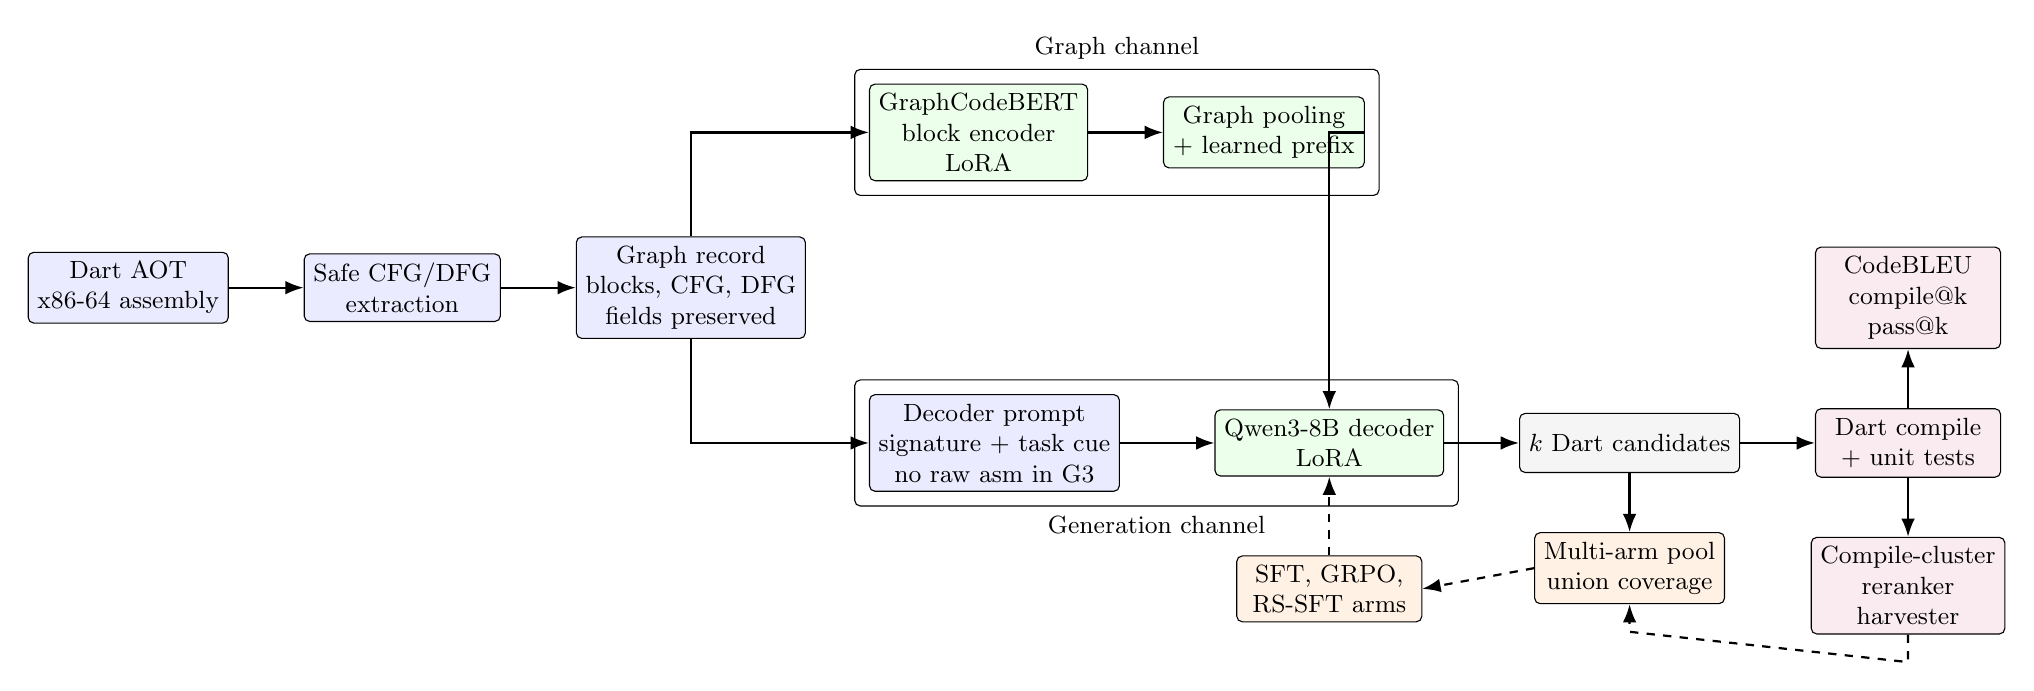
\begin{tikzpicture}[
  font=\small,
  >=Latex,
  node distance=0.75cm and 0.95cm,
  box/.style={draw, rounded corners=2pt, align=center, minimum height=0.75cm, minimum width=2.2cm, fill=gray!8},
  data/.style={draw, rounded corners=2pt, align=center, minimum height=0.75cm, minimum width=2.35cm, fill=blue!8},
  model/.style={draw, rounded corners=2pt, align=center, minimum height=0.82cm, minimum width=2.55cm, fill=green!8},
  train/.style={draw, rounded corners=2pt, align=center, minimum height=0.75cm, minimum width=2.35cm, fill=orange!10},
  eval/.style={draw, rounded corners=2pt, align=center, minimum height=0.75cm, minimum width=2.35cm, fill=purple!8},
  arrow/.style={->, thick},
  dasharrow/.style={->, thick, dashed}
]

\node[data] (asm) {Dart AOT\\x86-64 assembly};
\node[data, right=of asm] (extract) {Safe CFG/DFG\\extraction};
\node[data, right=of extract] (graph) {Graph record\\blocks, CFG, DFG\\fields preserved};

\node[model, above right=0.7cm and 0.8cm of graph] (encoder) {GraphCodeBERT\\block encoder\\LoRA};
\node[model, right=of encoder] (pool) {Graph pooling\\+ learned prefix};

\node[data, below right=0.7cm and 0.8cm of graph] (prompt) {Decoder prompt\\signature + task cue\\no raw asm in G3};
\node[model, right=1.2cm of prompt] (decoder) {Qwen3-8B decoder\\LoRA};
\node[box, right=of decoder] (cands) {$k$ Dart candidates};

\node[eval, right=of cands] (harness) {Dart compile\\+ unit tests};
\node[eval, above=of harness] (metrics) {CodeBLEU\\compile@k\\pass@k};
\node[eval, below=of harness] (rerank) {Compile-cluster\\reranker\\harvester};

\node[train, below=1.0cm of decoder] (adapt) {SFT, GRPO,\\RS-SFT arms};
\node[train, below=of cands] (ensemble) {Multi-arm pool\\union coverage};

\draw[arrow] (asm) -- (extract);
\draw[arrow] (extract) -- (graph);
\draw[arrow] (graph) |- (encoder);
\draw[arrow] (encoder) -- (pool);
\draw[arrow] (pool) -| (decoder);
\draw[arrow] (graph) |- (prompt);
\draw[arrow] (prompt) -- (decoder);
\draw[arrow] (decoder) -- (cands);
\draw[arrow] (cands) -- (harness);
\draw[arrow] (harness) -- (metrics);
\draw[arrow] (harness) -- (rerank);
\draw[arrow] (cands) -- (ensemble);
\draw[dasharrow] (ensemble.west) -- (adapt.east);
\draw[dasharrow] (adapt) -- (decoder);
\coordinate (rerankDrop) at ($(rerank.south)+(0,-0.35)$);
\coordinate (ensembleDrop) at ($(ensemble.south)+(0,-0.35)$);
\draw[dasharrow] (rerank.south) -- (rerankDrop) -- (ensembleDrop) -- (ensemble.south);

\node[draw, rounded corners=2pt, fit=(encoder) (pool), inner sep=0.18cm, label={[font=\small]above:Graph channel}] {};
\node[draw, rounded corners=2pt, fit=(prompt) (decoder), inner sep=0.18cm, label={[font=\small]below:Generation channel}] {};
\end{tikzpicture}%
}
\caption{Overview of the graph-conditioned Dart AOT decompilation pipeline. The graph path extracts CFG/DFG structure and bounded per-block instructions from assembly and encodes them with a LoRA-adapted GraphCodeBERT encoder. Learned prefix tokens condition a LoRA-adapted Qwen3-8B decoder; RMS matching is evaluated separately as a stability mechanism for wider prefix variants. Generated Dart candidates are evaluated by compile and test harnesses; the same candidate pools support GRPO rewards, rejection-sampling SFT, reranking, and multi-arm union analysis.}
\label{fig:architecture}
\end{figure}

Figure~\ref{fig:architecture} summarizes the architecture and evaluation loop. The key design choice is to avoid treating the assembly listing as another long decoder prompt. G3 is not a topology-only model: the graph/local block encoder consumes bounded per-block assembly instructions together with CFG/DFG relationships, compresses them into learned prefix tokens, and leaves only the function-level task cue in the causal decoder prompt.

\subsection{Task and data}

The study contains two historically distinct corpora, not a 126-task subset of HumanEval-Dart. The primary functional corpus has 154 filtered, test-equipped HumanEval-Dart functions with signatures, reference Dart implementations, AOT-derived x86-64 assembly, CFG/DFG-derived graph features, and unit tests. It supports pass@k and the aligned JIT/pass-harness compile@k used in the main results. The older 126-row corpus contains standalone Dart programs and reference sources from the earlier CodeBLEU/standalone-compile workflow; its rows are mostly top-level \texttt{main} programs, do not contain the HumanEval test field, and share no filenames with the 154-task corpus. We retain that separate corpus only for CodeBLEU and historical comparison in Appendix~\ref{app:legacycompile}. It is not evidence that 28 HumanEval-Dart tasks were excluded from a larger set.

\subsection{Graph extraction}

The graph pipeline extracts basic blocks from assembly using jump targets and fall-through structure, control-flow edges between blocks, lightweight data-flow edges tracking register/value relationships where available, and per-block instruction summaries with bounded instruction counts. The graph records are merged into the original JSONL rows without dropping fields such as \texttt{dart\_source}, \texttt{tests}, \texttt{dart\_function\_signature}, and \texttt{assembly}. This is important because earlier conversion code could create graph-only records and accidentally destroy the SFT/GRPO fields required by training and evaluation.

\subsection{Model architecture}

The best clean architecture uses GraphCodeBERT as the graph/local block encoder, Qwen3-8B as the causal decoder, learned graph prefix tokens injected into the decoder context, and LoRA on both encoder and decoder with rank 64 and alpha 128. Prefix RMS matching is reported as a stability mechanism for the wide-prefix ablation, not as an assumed property of the archived 16-prefix G3 row.

The primary graph-conditioned configuration is given below. Each entry is a single runner parameter written as \texttt{key = value} in \texttt{snake\_case}, matching the released code:

\begin{table}[h]
\centering
\small
\begin{tabular}{@{}ll@{}}
\toprule
Parameter & Value \\
\midrule
\texttt{qwen\_prefix\_tokens} & \texttt{16} \\
\texttt{qwen\_prefix\_rms\_match} & \texttt{0} (for the reported 16-prefix G3 row) \\
\texttt{prompt\_assembly\_mode} & \texttt{"none"} \\
\texttt{prompt\_fit\_assembly} & \texttt{1} (inert when \texttt{prompt\_assembly\_mode = "none"}) \\
\texttt{dfg\_mode} & \texttt{"edges"} \\
\texttt{position\_scheme} & \texttt{"roberta"} \\
\texttt{auto\_cfg} & \texttt{0} \\
\texttt{max\_block\_instrs} & \texttt{24} \\
\texttt{graph\_max\_dataflow\_edges} & \texttt{4096} \\
\bottomrule
\end{tabular}
\end{table}

The \texttt{prompt\_assembly\_mode = "none"} setting is deliberate: the model receives structure through the graph channel rather than duplicating long assembly text in the decoder prompt. The RMS-matched p128r arm instead uses \texttt{qwen\_prefix\_rms\_match = 1}.

\subsection{Adaptation arms}

We evaluate null and text-only controls, graph-text and CFG-only variants, the clean graph-only G3 architecture, wider prefix variants, GRPO reward tuning with binary/full-pass reward variants, RS-SFT from all passing candidates harvested across arms, and ultralite repair arms from GRPO, RS-SFT, and style-SFT checkpoints. Our aim is not to identify a universally dominant checkpoint, but to characterize how each intervention shifts the tradeoff among CodeBLEU, compilability, and functional correctness.

\subsection{Reranking and ensembling}

We distinguish intra-model reranking from multi-arm candidate ensembling. Intra-model reranking generates k candidates from one checkpoint and selects one candidate with deployable heuristics. Multi-arm candidate ensembling pools candidates from multiple independently adapted checkpoints, then measures union coverage or reranks over the pool. The deployable reranker, \texttt{compile\_cluster\_vote}, uses Dart compilation, structural heuristics, and candidate clustering. It does not use hidden tests. Oracle reranking uses pass/fail outcomes only to estimate the upper bound available in a sampled candidate pool.

\section{Experimental Setup}

All main experiments use the exact \texttt{Qwen/Qwen3-8B} checkpoint as decoder and GraphCodeBERT as encoder. The \emph{base reference} row is the untuned Qwen3-8B decoder given the cleaned assembly prompt under the same evaluator and sampling protocol, with the learned graph-prefix channel disabled. Unless otherwise stated, the primary 154-task pass/aligned-compile evaluation uses 10 samples, maximum generation length 768 tokens, decoder prompt budget 2048 tokens, LoRA rank 64, alpha 128, and 16 graph prefix tokens. The separate 126-row CodeBLEU/legacy-compile workflow uses five samples. RMS matching is enabled only for runs whose labels or archived configurations explicitly include it, such as p128r.

For a task with \(n\) generated candidates and \(c\) passing candidates, pass@k follows the HumanEval estimator \(1 - \binom{n-c}{k}/\binom{n}{k}\), averaged over tasks \cite{chen2021codex}. We use the same convention for compile@k by replacing test pass with successful Dart front-end acceptance. When \(n=k\), as in pass@10 with ten samples and the historical compile@5 view with five samples, the estimator reduces to task coverage: whether at least one candidate succeeds. pass@1 and compile@1 reduce to \(c/n\) for each task before averaging.

Local multi-sample evaluation uses stochastic decoding with temperature 0.7 and nucleus sampling \(p=0.95\); single-sample evaluation is greedy. We report CodeBLEU on the separate 126-row reference corpus, aligned compile@5/compile@10 and pass@1/pass@5/pass@10 on the 154-task functional corpus, task-level union coverage across arms, and deployable/oracle reranking results.

\paragraph{Frontier baseline.} To calibrate all specialized results against current general-purpose capability, we additionally prompt four frontier models zero-shot on the same 154 tasks: an Azure \texttt{gpt-chat-latest} deployment identified by the provider as GPT-5.5, Claude Sonnet~5, DeepSeek~V4~Pro, and GLM-5.2, accessed through hosted APIs on July 8, 2026. Each model receives the full x86-64 AOT disassembly and the target function signature, with no graph channel, no fine-tuning, and no truncation to the 2048-token decoder budget used for the specialized models; the prompt is frozen after light calibration on five held-out tasks. This comparison is intentionally not architecture-controlled; it measures the capability available to a practitioner using a hosted frontier model at that date. Architecture-controlled comparisons within the 8B local regime are reported separately. The client makes ten independent requests per task with temperature 0.7, \(p=0.95\), and a 1{,}024-token output cap, and the archived per-row metadata records those requested controls. Empty content and request errors remain blank candidate slots and are scored as failures: 115/1{,}540 slots are blank for GPT-5.5, 765 for Sonnet~5, 1{,}233 for DeepSeek, and 1{,}188 for GLM. GPT-5.5 and Sonnet~5 have no recorded API-error rows; DeepSeek has three and GLM one, so most blank slots are empty provider responses rather than caught request exceptions. This is an end-to-end practitioner baseline under a fixed request budget, not a comparison conditioned on receiving ten non-empty programs. Because OpenRouter and Azure may translate, clamp, or ignore sampling fields internally, we do not claim that effective provider-side sampling was independently verified. The moving Azure alias is treated as a dated snapshot, not a permanently reproducible model identifier. Generations are scored by the identical Dart pass harness. The 154-task compile@k rows use a JIT/pass-harness compile definition: we run the same candidate-plus-tests file through \texttt{dart run}, count front-end syntax/type errors as compile failures, and count runtime assertion failures or timeouts as compiled-but-not-passing. This makes compile@k and pass@k nested on the same candidate pools; strict AOT compilation is retained only as an additional diagnostic because it rejects some programs accepted by the JIT pass harness.

\paragraph{GPT-5.5 prompt ablation.} We separately query the Azure GPT-5.5 deployment with seven prompt representations, ten candidates per task, an 8{,}192-token output cap, and deployment-default sampling shared by every ablation arm. The first serializer (\emph{v1}) supports full assembly, a character-estimated cap of approximately 2{,}048 assembly tokens, full assembly plus a compact CFG topology, and compact topology without block instructions. The cap applies to assembly text rather than to the total prompt; only 46/154 records have lower API-reported prompt-token counts than their full-assembly counterpart. That accounting check says which requests the heuristic changed; it is not an instruction-count threshold and should not be conflated with the local decoder's observed difficulty on long assembly. The revised serializer (\emph{v2}) removes GDB dump headers and uses the cleaned instruction stream in three matched conditions: cleaned assembly only, cleaned assembly plus an address-aligned CFG with final block instructions, and all normalized instructions organized inside their CFG blocks without a separate flat listing. The v2 conditions share the same cleaner, system prompt, Azure deployment, output cap, and deployment-default sampling, so their paired comparisons are controlled. Direct v1--v2 comparisons remain descriptive because the serializer revision also changes assembly cleaning and parts of the system prompt.

The main paper uses one compile definition: the 154-task JIT/pass-harness metric computed from the same candidate-plus-tests files as pass@k. This guarantees that pass@k is nested under compile@k. CodeBLEU and the earlier 126-task standalone-compile view are retained only as historical diagnostics in Appendix~\ref{app:legacycompile}; functional conclusions are based on pass@k.

\section{Results}

\subsection{Standalone model results}

\begin{table}[t]
\centering
\small
\caption{Standalone x86 8B results. CodeBLEU is a historical similarity diagnostic on the 126-task reference set; pass@k is measured on 154 HumanEval-Dart tasks and is the functional result. The archived experiment label is shown in \texttt{monospace}. The legacy standalone-compile values are moved to Appendix~\ref{app:legacycompile}.}
\label{tab:standalone}
\resizebox{\textwidth}{!}{%
\begin{tabular}{lrrrr}
\toprule
Arm & CodeBLEU & pass@1 & pass@5 & pass@10 \\
\midrule
Binary-reward GRPO \texttt{(binary GRPO)} & 0.5438 & 0.0409 & 0.1280 & 0.1818 \\
Rejection-sampling SFT, all arms \texttt{(RS-SFT all-arms)} & 0.5740 & 0.0474 & 0.1296 & 0.1688 \\
Rejection-sampling SFT, reference \texttt{(binary RS-SFT ref)} & 0.5323 & 0.0357 & 0.1121 & 0.1558 \\
Graph-conditioned (16 prefix) \texttt{(clean G3)} & 0.6383 & 0.0266 & 0.0996 & 0.1558 \\
Style-SFT repair \texttt{(style repair ultralite)} & 0.5299 & 0.0240 & 0.0918 & 0.1429 \\
Graph-conditioned, 128 prefix + RMS \texttt{(G3 p128r)} & 0.6349 & 0.0292 & 0.0878 & 0.1364 \\
Style-SFT (1{,}036 ex.) \texttt{(style1036 SFT)} & 0.5709 & 0.0325 & 0.0972 & 0.1364 \\
CFG-only conditioning \texttt{(CFG-only)} & 0.6063 & 0.0201 & 0.0671 & 0.1104 \\
Pass@k-oriented GRPO \texttt{(SimKO-style GRPO)} & 0.6360 & 0.0221 & 0.0716 & 0.1104 \\
Serialized graph-in-prompt \texttt{(graph-text)} & 0.6253 & 0.0227 & 0.0691 & 0.0974 \\
Untuned Qwen3-8B \texttt{(base reference)} & 0.5383 & 0.0156 & 0.0563 & 0.0909 \\
Null-graph control \texttt{(null graph)} & 0.5459 & 0.0136 & 0.0494 & 0.0779 \\
Text-only control \texttt{(text-only)} & 0.5193 & 0.0052 & 0.0260 & 0.0519 \\
Graph-conditioned, 128 prefix, no RMS \texttt{(p128 without RMS)} & 0.4481 & 0.0000 & 0.0000 & 0.0000 \\
\bottomrule
\end{tabular}
}
\end{table}

The archived experiment-family labels shown in \texttt{monospace} parentheses map to the released artifact: \texttt{G3} is the clean graph-conditioned architecture, \texttt{p128r} its 128-prefix RMS-matched variant, \texttt{style1036} the style-matched synthetic SFT arm, and \texttt{ref}, \texttt{lite}, and \texttt{ultralite} the harvested repair-set variants used for quick consolidation checks. Appendix~\ref{app:labels} gives the full label-to-configuration mapping.

Among the specialized arms, clean G3 has the strongest CodeBLEU, while binary GRPO has the highest pass@10. Under the primary aligned compile definition in Table~\ref{tab:frontier}, GRPO and clean G3 are close at compile@5 (0.403 versus 0.422). No specialized arm is uniformly best once CodeBLEU is treated as a diagnostic: G3 leads on similarity and GRPO leads on functional pass@k.

\subsection{Frontier baseline comparison}
\label{sec:frontier}

Table~\ref{tab:frontier} places the specialized arms against four frontier models prompted zero-shot on the same assembly. The gap at the top is large. The dated GPT-5.5 snapshot reaches pass@10 of 0.701, roughly four times the best specialized arm (0.182) and more than twice the 17-arm union coverage (0.279). Claude Sonnet~5 (0.487) and DeepSeek~V4~Pro (0.351) also clearly exceed the union; GLM-5.2 (0.286) edges it by one covered task, 44 versus 43, so we do not interpret that last difference as a meaningful capability gap. On aligned JIT/pass-harness compile the frontier rows remain strong: GPT-5.5 reaches compile@10 of 0.955, while clean G3 and binary GRPO reach 0.630 and 0.591 respectively. None of the frontier models received any decompilation-specific training, graph conditioning, or Dart AOT adaptation. For HumanEval-scale Dart AOT functions, then, general frontier capability currently dominates the specialized 8B pipeline on functional correctness, and the specialized interventions studied here should be read as characterizing the small-local-model regime rather than as competitive with hosted frontier inference.

\begin{table}[t]
\centering
\small
\caption{Frontier models (zero-shot, full assembly, no graph channel) versus specialized arms on the 154-task pass set. compile@k uses the primary JIT/pass-harness definition on the same candidate-plus-tests files as pass@k, so pass@k is nested under compile@k. Empty or failed hosted responses remain failed sample slots. Best in each column is in \textbf{bold}.}
\label{tab:frontier}
\resizebox{\textwidth}{!}{%
\begin{tabular}{lrrrrr}
\toprule
Model / arm & compile@5 & compile@10 & pass@1 & pass@5 & pass@10 \\
\midrule
\multicolumn{6}{l}{\emph{Frontier models, zero-shot}} \\
GPT-5.5 & \textbf{0.9495} & \textbf{0.9545} & \textbf{0.5526} & \textbf{0.6709} & \textbf{0.7013} \\
Claude Sonnet 5 & 0.6365 & 0.6818 & 0.3058 & 0.4358 & 0.4870 \\
DeepSeek V4 Pro & 0.5164 & 0.6753 & 0.0851 & 0.2561 & 0.3506 \\
GLM-5.2 & 0.3660 & 0.4286 & 0.1461 & 0.2526 & 0.2857 \\
\midrule
\multicolumn{6}{l}{\emph{Specialized arms (this work), 154-task JIT/pass-harness compile}} \\
Binary-reward GRPO & 0.4033 & 0.5909 & 0.0409 & 0.1280 & 0.1818 \\
Graph-conditioned (clean G3) & 0.4215 & 0.6299 & 0.0266 & 0.0996 & 0.1558 \\
All-arm union (17 arms) & -- & -- & -- & -- & 0.2792 \\
Untuned Qwen3-8B & 0.2207 & 0.3701 & 0.0156 & 0.0563 & 0.0909 \\
\bottomrule
\end{tabular}
}
\end{table}

\subsection{GPT-5.5 context and graph-serialization ablations}

Table~\ref{tab:gptablation} tests whether the frontier gap can be attributed primarily to GPT-5.5 seeing a longer assembly prompt, and whether a textual CFG helps the frontier model. This is a separate Azure run from the canonical GPT-5.5 row in Table~\ref{tab:frontier}: it uses an 8{,}192-token output cap and deployment-default sampling, so its full-assembly row is the within-ablation control rather than a replacement for the main frontier estimate. Its 110-task full-assembly coverage (0.7143) is two tasks above the canonical run's 108 (0.7013), but the pools differ in output cap and sampling protocol; we treat that difference as between-run variation, not as an improvement attributable to any prompt representation.

\begin{table}[t]
\centering
\small
\caption{GPT-5.5 prompt-representation ablation on the same 154 tasks, with ten candidates per task. \emph{Covered} is the pass@10 numerator. Within-version comparisons are controlled; direct v1--v2 comparisons remain descriptive because the cleaner and system prompt changed.}
\label{tab:gptablation}
\resizebox{\textwidth}{!}{%
\begin{tabular}{llrrrr}
\toprule
Prompt condition & Pipeline & pass@1 & pass@5 & pass@10 & Covered \\
\midrule
Full assembly & v1 & 0.5851 & 0.6894 & 0.7143 & 110 \\
Approx. 2{,}048-token assembly cap & v1 & 0.5721 & 0.6718 & 0.7013 & 108 \\
Assembly + compact CFG topology & v1 & 0.5864 & 0.6910 & \textbf{0.7273} & \textbf{112} \\
Compact CFG topology only & v1 & 0.3935 & 0.4800 & 0.5065 & 78 \\
\midrule
Cleaned assembly only & v2 & 0.5792 & 0.6789 & 0.7078 & 109 \\
Clean assembly + address-aligned CFG & v2 & 0.5695 & 0.6729 & 0.7013 & 108 \\
CFG-organized block instructions, no flat listing & v2 & 0.5656 & 0.6774 & 0.7013 & 108 \\
\bottomrule
\end{tabular}
}
\end{table}

Within v1, the approximate assembly cap covers 108 tasks versus 110 for full assembly, with three tasks gained and five lost (exact two-sided McNemar \(p=0.727\)). The observed frontier advantage therefore is not explained primarily by this context-budget difference. Adding the compact CFG topology raises the point estimate to 112 tasks, but the paired difference is also non-significant (\(+3/-1\), \(p=0.625\)); the data do not establish that textual CFG augmentation improves GPT-5.5. Removing block contents and providing only the compact topology reduces coverage to 78 tasks (\(+5/-37\), \(p=4.43{\times}10^{-7}\)). This last result shows that the particular topology-only textual summary is lossy; it does not imply that raw assembly should be fed directly to a smaller decoder.

Within v2, cleaned assembly alone covers 109 tasks. Adding the address-aligned CFG covers 108, with two tasks gained and three lost relative to cleaned assembly (exact two-sided McNemar \(p=1.000\)); organizing all instructions inside CFG blocks also covers 108 (\(+1/-2\), \(p=1.000\)). The corresponding aligned compile@10 values are 0.9870, 0.9675, and 0.9805. Thus neither v2 textual graph representation improves GPT-5.5 over the matched cleaned-assembly control, although CFG organization preserves nearly all functional and compile coverage while eliminating the separate flat listing.

That distinction is central to the local architecture. G3 is called graph-only because raw assembly is absent from the Qwen decoder prompt, not because instructions are discarded. Its GraphCodeBERT/local-block path consumes bounded block instructions and graph relationships before compressing them into 16 learned prefix tokens. Conversely, the v2 \emph{CFG-organized block instructions} condition still contains every normalized instruction, merely grouped by block instead of repeated as a flat listing. The controlled v2 result therefore argues against claiming that textual CFG organization helps a frontier model, but it does not test the learned graph-prefix compression used by G3 or imply that raw assembly is suitable for a much smaller decoder.

\begin{table}[t]
\centering
\scriptsize
\caption{Task-level pass@10 uncertainty and paired tests for selected comparisons. Coverage intervals are Wilson 95\% confidence intervals. Paired tests are exact two-sided McNemar tests against clean G3; \(+g/-l\) reports tasks gained/lost on the same 154 benchmark rows. The all-arm union is a budget-unmatched coverage diagnostic.}
\label{tab:paired}
\resizebox{\textwidth}{!}{%
\begin{tabular}{lrr}
\toprule
Arm & pass@10 (95\% CI) & McNemar \\
\midrule
clean G3 graph-only & 0.1558 [0.1070, 0.2214] & -- \\
binary GRPO & 0.1818 [0.1289, 0.2502] & \mcnemar{7}{3}{0.344} \\
RS-SFT all-arms & 0.1688 [0.1179, 0.2359] & \mcnemar{7}{5}{0.774} \\
CFG-only & 0.1104 [0.0701, 0.1697] & \mcnemar{5}{12}{0.143} \\
text-only & 0.0519 [0.0266, 0.0992] & \mcnemar{2}{18}{4.0{\times}10^{-4}} \\
p128 without RMS & 0.0000 [0.0000, 0.0243] & \mcnemar{0}{24}{1.2{\times}10^{-7}} \\
all-arm union & 0.2792 [0.2144, 0.3548] & \mcnemar{19}{0}{3.8{\times}10^{-6}} \\
\bottomrule
\end{tabular}
}
\end{table}

Table~\ref{tab:paired} shows why the point estimates should not be overread. Binary GRPO has the largest standalone specialized pass@10 numerator, but its paired gain over clean G3 is small and not statistically distinguishable at this sample size. Applying Holm--Bonferroni correction across the six pass@10 comparisons preserves the p128 collapse (\(p_{\mathrm{Holm}}=7.2{\times}10^{-7}\)), the text-only regression (\(p_{\mathrm{Holm}}=1.6{\times}10^{-3}\)), and the all-arm coverage gain (\(p_{\mathrm{Holm}}=1.9{\times}10^{-5}\)); binary GRPO (\(p_{\mathrm{Holm}}=0.688\)), RS-SFT (0.774), and CFG-only (0.429) remain non-significant. These analyses were not preregistered and come from fixed archived generation pools rather than repeated training seeds, so the p-values are task-level diagnostics rather than evidence of training-run stability. The union adds 19 tasks without losing a clean-G3-covered task, but it uses a much larger candidate budget (17 arms $\times$ 10 samples versus 10 samples). It is therefore a candidate-discovery ceiling, not a fair deployment comparison; we return to this asymmetry in Section~\ref{sec:ensemble}.

\subsection{Architecture ablations}

The graph-conditioned arms have higher pass@10 than the text-only and null controls in these fixed runs. Clean G3 reaches 0.1558, compared with 0.0519 for the text-only G1 arm and 0.0779 for the null graph. This comparison is about representation, not topology replacing semantics. G1 sends the full cleaned assembly listing through the causal decoder prompt with no graph prefix, whereas G3 removes raw assembly from that prompt but still encodes bounded instructions inside each basic block together with graph edges. The threefold observed difference is consistent with the small decoder benefiting from learned structure-aware compression into 16 prefix tokens; without repeated training seeds, it is not an estimate of training-run variance and does not establish that CFG topology alone would suffice.

The current ablations do not prove that DFG edges help on their own. CFG-only outperforms graph-text on pass@10 (0.1104 versus 0.0974), and these rows do not isolate DFG under the same graph-only regime as G3. We therefore interpret the result as evidence for graph conditioning overall, while treating DFG contribution as unresolved and requiring a future controlled ablation.

The p128 experiment shows that simply increasing prefix capacity is unsafe. Without RMS matching, the 128-prefix variant collapses to zero pass@k and very low compile@5. With RMS matching, p128r recovers compile@5 and CodeBLEU but still underperforms the 16-prefix G3 model on pass@10. The lesson is that graph-prefix scale and conditioning stability matter more than raw prefix width.

\subsection{GRPO and RS-SFT}

GRPO reaches standalone pass@10 of 0.1818, the highest observed value among the specialized arms, while aligned compile@5 is close to clean G3 (0.403 versus 0.422). Its paired pass@10 difference from clean G3 is not significant. RS-SFT all-arms has higher pass@1 and pass@5 point estimates than clean G3 but lower CodeBLEU. Attempts to repair GRPO with RS-SFT wash out the useful pass@10 tail in these archived runs.

This supports a careful interpretation: correctness rewards can move probability mass toward passing solutions, but the setting is small and sparse. GRPO optimizes expected per-sample reward, whereas pass@k rewards the existence of diverse correct candidates in the tail. The objectives are related but not identical. We no longer characterize GRPO as simply ``unstable'': on functional metrics it is the strongest specialized arm, and its earlier apparent compile fragility is an artifact of the legacy standalone-compile metric.

\subsection{Multi-arm candidate ensembling}
\label{sec:ensemble}

The largest task-level coverage gain is observed when candidates are pooled across independently adapted arms, although this result reflects candidate-set complementarity rather than single-model generalization. Across 17 prediction files, 43/154 tasks have at least one passing candidate, 111/154 tasks remain zero-pass, 587 passing candidates are found before deduplication, 142 RS-SFT rows remain after dedupe and per-task capping, and 253 rows are available in the all-plus-reference RS-SFT set. The multi-arm pool combines the 14 primary model families in Table~\ref{tab:standalone} with three auxiliary repair/rerank pools; the exact auxiliary labels are retained here for traceability: \texttt{withB ref lite}, \texttt{withB ref ultralite}, and \texttt{binary repair ultralite}.

This is substantially higher than the clean G3 single-arm coverage of 24 tasks and the best GRPO single-arm coverage of 28 tasks. These are candidate-coverage counts (tasks with at least one passing sample); the corresponding pass@10 estimates in Table~\ref{tab:standalone} are 0.156 and 0.182. The comparison is not sample-budget matched: the union pools many more candidates than a single 10-sample arm. We therefore interpret it as a coverage ceiling and diversity diagnostic, not as evidence that a 17-arm system is the deployable default. The multi-arm result shows that the models fail differently. Even weak standalone arms can add new tasks to the union. The H100 ultralite label denotes a run group executed on H100 hardware, not a distinct algorithm; those arms added three new tasks to the union: \texttt{List<int> unique(List<int> list)}, \texttt{bool correctBracketing(String brackets)}, and \texttt{bool primeLength(String string)}. This complementarity motivates treating candidate ensembling as a first-class inference-time method rather than as an afterthought.

\subsection{Reranking}

\begin{table}[t]
\centering
\small
\caption{Deployable compile-cluster reranking on recent H100 arms. Rates are measured on the 154-task pass-set candidate pools, not the 126-task compile/CodeBLEU set. Orig. denotes the first/original candidate, Sel. denotes the compile-cluster-selected candidate, and Oracle pass denotes a hidden-test upper-bound diagnostic.}
\label{tab:rerank}
\resizebox{\textwidth}{!}{%
\begin{tabular}{lrrrrr}
\toprule
Arm & Orig. comp. & Sel. comp. & Orig. pass & Sel. pass & Oracle pass \\
\midrule
Reference repair, small \texttt{(withB ref lite)} & 0.0584 & 0.4351 & 0.0130 & 0.0325 & 0.0519 \\
Reference repair, smallest \texttt{(withB ref ultralite)} & 0.0909 & 0.4351 & 0.0130 & 0.0584 & 0.0779 \\
Binary-reward repair \texttt{(binary repair ultralite)} & 0.0649 & 0.4026 & 0.0000 & 0.0844 & 0.1104 \\
Style-SFT repair \texttt{(style repair ultralite)} & 0.0779 & 0.3442 & 0.0260 & 0.0844 & 0.1364 \\
\bottomrule
\end{tabular}
}
\end{table}

The archived labels in Table~\ref{tab:rerank} (\texttt{withB} denoting B-sweep harvest/repair candidate pools, \texttt{lite}/\texttt{ultralite} the smaller repair sets) are retained in parentheses so the table can be traced back to the released result files; see Appendix~\ref{app:labels}.

Deployable compile-cluster reranking improves selected compile rates substantially, as shown in Table~\ref{tab:rerank}. The deployable reranker does not reach the oracle ceiling, but it materially improves selection. The oracle gap quantifies how much additional benefit would require better semantic selection or public tests. More importantly, for several weak arms, the reranker recovers enough compile behavior to make their candidate pools useful for downstream harvesting and analysis.

The large compile jump should be read as a reranking effect, not as a new model compile@1 probability: the reranker chooses among an existing sampled pool, so selected compile can be much higher than the original first-candidate compile rate.

\section{Discussion}

\subsection{What graph conditioning buys}

Graph conditioning improves the similarity profile and moves the model beyond text-only decoding: G3 has the strongest CodeBLEU among the specialized arms and competitive functional scores. Its benefit should be read as learned compression of local instruction content and graph relationships, not as evidence that bare topology is sufficient. This matters because the text-only 8B arm performs poorly when the causal decoder must consume the full assembly directly, while G3 encodes bounded block contents outside that prompt. We are careful not to overstate the result. Once CodeBLEU is treated as a diagnostic, G3 does not dominate the reward-tuned arms on functional metrics, and its earlier ``best balanced'' status rested partly on the legacy standalone-compile metric. The defensible claim is narrower than in an earlier draft: within the small-local-model regime, graph conditioning is a reasonable default that trades a little functional pass@k for markedly better similarity and a compact decoder context, but it is not the single best specialized configuration on functional grounds, and it is far from frontier capability.

\subsection{Frontier models versus specialized small models}

The frontier comparison is the result with the largest practical consequence. A general model with no decompilation-specific training recovers functionally correct Dart several times more often than any specialized arm; Claude Sonnet~5 and DeepSeek~V4~Pro also exceed the full multi-arm union, while GLM-5.2 is separated from it by only one task. The GPT-5.5 prompt ablation narrows the explanation: reducing assembly with a character-estimated 2{,}048-token cap changes coverage from 110 to 108 tasks and is not significant in the paired test. The observed gap therefore is not explained by this particular cap on the affected rows, although the experiment is not an exact total-prompt-budget control. Parameter and pretraining scale, broad exposure to Dart and assembly-like text, and stronger in-context semantic reconstruction remain plausible explanations rather than measured causal factors. Similarly, the compact textual CFG condition has the highest point estimate in the ablation but no significant paired advantage, so we do not claim that simply appending serialized topology improves a frontier model. The honest reading is that, for HumanEval-scale Dart AOT functions, specialized 8B training does not currently buy accuracy over a frontier zero-shot call.

This does not make specialized models pointless, but it relocates their value. The decompilation targets that motivate this work -- proprietary Flutter binaries, malware, regulated or air-gapped code -- are frequently exactly the inputs that cannot be sent to a hosted frontier API. In that regime the relevant comparison is not frontier-versus-specialized but specialized-versus-nothing, and a local model that runs offline at controlled cost has a genuine niche. The frontier numbers also point to the most promising way to raise the specialized ceiling: distillation, using frontier models as teachers to generate large, correct Dart AOT training corpora for small deployable students, rather than reward-tuning a small model against sparse signals. We therefore frame the specialized contributions here as characterizing and partially narrowing a gap that distillation, not on-policy reward optimization, is best placed to close.

\subsection{Why reward tuning is not a shortcut}

The GRPO arm has the highest specialized pass@10, and under aligned JIT/pass-harness compile it no longer looks fragile. But it does not close the frontier gap, and its gains over graph conditioning are not statistically separable at this sample size. The likely dynamics are familiar: in a group-normalized sparse-reward setting, a rare full-pass response receives a large positive advantage while most responses receive little useful semantic signal, so probability mass concentrates around a few discovered patterns. This improves candidate discovery for some tasks without producing a broadly stronger decompiler. The practical role of GRPO in this setting is as a candidate-discovery arm feeding the union, not as a standalone deployable checkpoint and not as a substitute for stronger base models or distilled data.

\subsection{Why ensembling matters}

pass@k is a coverage metric. If different adaptation strategies solve different tasks, then a multi-arm ensemble can reveal a larger recoverable set than any single model. The union result, 43/154, demonstrates that several apparently weak arms are still scientifically valuable because they contribute unique passing candidates.

\subsection{Reranking as a bridge between research and deployment}

Oracle reranking measures the sampled pool ceiling; deployable reranking tries to approximate it using available signals. Our compile-cluster reranker strongly improves selected compile rates but only partially improves selected pass@1. This suggests a clear next step: semantic rerankers that do not require hidden tests, such as learned failure predictors, signature/type consistency models, lightweight symbolic checks, or public-example execution when available.

\section{Artifact and Reproducibility Notes}

The public reproducibility bundle is released at \url{https://github.com/raafatabualazm/MSc-Code/tree/graph-decompiler-2026-v1/graph_decompiler_2026_artifact}. It contains the graph extraction, GraphCodeBERT/Qwen3-8B training, GRPO, RS-SFT, evaluation, statistical-analysis, and reranking code; the two benchmark JSONL files and their schemas; run configurations and command history; raw local-arm and frontier predictions; per-candidate metrics; aggregate summaries; and the paper source. The seven GPT-5.5 ablation pools in Table~\ref{tab:gptablation} retain prompt mode and token accounting, and the v2 pools additionally retain exact prompt hashes and serializer-version metadata. Their aggregate and paired results are consolidated in \texttt{frontier/GPT55Abl/gpt55\_ablation\_summary.json}.

The reported 8B adapter collection is hosted separately at \url{https://huggingface.co/raafatabualazm/antigravity-qwen3-8b-artifacts}. The release manifest pins Hugging Face repository revision \texttt{bc992cecbb6968be2e20b6e99e8a4c420e32242c} and records each hosted file's LFS SHA-256 identifier, size, and path. This avoids claiming that locally absent multi-gigabyte files were hashed after the fact. The Git bundle also includes a SHA-256 manifest for every released local file and the captured local verification environment (Python 3.12.7; \texttt{torch} 2.11.0+cu128, \texttt{transformers} 5.9.0, \texttt{peft} 0.18.0, \texttt{torch-geometric} 2.7.0, \texttt{accelerate} 1.6.0), plus the offline preprocessing and GRPO self-check suites.

Two reproducibility gaps remain explicit. The ephemeral training-pod package environment was not captured before the pods were destroyed; \texttt{training\_args.bin}, runner configurations, local verification pins, and model hashes are available, but they are not equivalent to a pod-side \texttt{pip freeze}. In addition, the literal interactive training invocations for four auxiliary repair pools used only in the reranking/union analysis (\texttt{withB ref lite}, \texttt{withB ref ultralite}, \texttt{binary repair ultralite}, and \texttt{style repair ultralite}) were not preserved. Their predictions and metrics are released, but these four pools are not presented as independently reproducible training arms and do not support the core G3-versus-control comparison.

The reported runs are exploratory rather than seed-averaged. We therefore treat cross-arm comparisons as task-level evidence from fixed sampled pools rather than as estimates over random training seeds. Representative GRPO sweeps use grouped rollouts, Dart compile/test rewards, LoRA rank 64 with alpha 128, and maximum rollout lengths between 512 and 768 tokens depending on the arm. The confidence intervals and pass@10 McNemar tests in Table~\ref{tab:paired} are recomputed from archived task-level outcomes, with the corrected paired-count artifact stored under \texttt{results/pass154\_same\_pools/}. Repeated training seeds and a captured pod environment remain requirements for a confirmatory follow-up.

\section{Threats to Validity}

Dataset size remains small: 154 pass@k tasks are enough to expose failure patterns but not enough to claim deployment readiness. The confidence intervals in Table~\ref{tab:paired} are task-level intervals over one archived generation pool, not seed-level uncertainty over retraining. Several training and evaluation arms share data, so harvest and ensemble results should be treated as optimization/coverage analysis rather than clean generalization. Some synthetic data is style-matched, but synthetic distributions may not reflect production Flutter binaries. The graph extractor is lightweight and may miss important data-flow relationships; DFG benefit is not isolated in a graph-only controlled ablation. The benchmark consists of short public HumanEval-derived functions, and the target signature itself may identify or strongly cue familiar tasks. We did not run a signature-only control, so frontier results measure practitioner-visible capability on this public benchmark rather than binary-derived semantic recovery in isolation. Finally, oracle reranking uses test outcomes and is not deployable unless those tests are public; it is reported only as an upper bound on candidate-pool quality.

Five caveats attach specifically to the frontier comparison. First, the frontier models are proprietary and versioned. The Azure \texttt{gpt-chat-latest} name is a moving alias, so the frontier rows are a July 8, 2026 snapshot rather than a permanently pin-able benchmark. Second, the requests record temperature and top-p, but effective provider-side sampling cannot be audited; OpenRouter's acceptance of the Sonnet~5 requests establishes successful transport, not that Anthropic applied those controls exactly. Third, the aligned JIT/pass-harness compile@k in Table~\ref{tab:frontier} answers whether the candidate is accepted by the same \texttt{dart run} front end used for pass@k, whereas strict AOT compilation can reject otherwise runnable programs. We therefore keep strict AOT compile as a diagnostic artifact rather than mixing it with pass@k in the main comparison. Fourth, the frontier comparison is a practitioner baseline, not an architecture-controlled comparison: model scale, training data, serving stack, and output budget differ from the local 8B system. The GPT-5.5 cap experiment addresses only one component and uses a character-estimated assembly cap rather than an exact 2{,}048-token total prompt; only 46 records show reduced API token accounting. Fifth, comparisons within v1 and within v2 are controlled, but direct v1--v2 comparisons are not because v2 changes disassembly cleaning and system-prompt wording in addition to graph serialization. These limitations do not affect the within-version paired tests.

\section{Dual-Use Considerations}

Neural decompilation supports legitimate reverse engineering, malware analysis, vulnerability research, interoperability, and software maintenance, but it can also lower the cost of inspecting proprietary code or adapting malicious binaries. Our release contains only generated benchmark programs, derived benchmark assembly/graphs, model adapters, and evaluation tooling; it contains no proprietary application binary, private source tree, credentials, exploit chain, or malware sample. The artifact documentation requires users to respect software licenses, authorization boundaries, and applicable law, and frames the system for reproducible research and defensive analysis. We release candidate generators rather than claiming a production decompiler: the low functional coverage, short-function benchmark, and need for external verification are prominently documented to reduce false confidence in security decisions. These controls cannot prevent all misuse, but they limit the release to materials necessary to validate the scientific claims while avoiding operational target data.

\section{Future Work}

The frontier comparison reshapes the priorities for future work. The most promising direction is distillation: using frontier models as teachers to generate large, correct, optimization-diverse Dart/Flutter AOT corpora, then training small deployable students on that data rather than reward-tuning them against sparse signals. Two existing artifacts make this a concrete next step rather than a purely speculative agenda. First, the released clean synthetic pool contains 1{,}726 source/assembly pairs with executable unit tests; it can support leakage-safe held-out distillation, rejection-sampling SFT, and reward experiments at substantially larger scale than the 154-task benchmark. Second, the stage-one ARM64 Flutter artifact contains 1{,}714 test-equipped release-build function slices with extracted CFGs. It establishes an ARM64 data and graph-extraction path, but its controlled semantics do not yet constitute evidence on production application logic. The next cross-ISA study should create fixed train/held-out splits, repeat the graph-versus-text ablation on ARM64, and test whether the learned compression transfers beyond x86-64. Complementary directions are larger and more realistic Dart/Flutter AOT datasets; optimization-matched Swift and Dart cross-lingual experiments; learned semantic rerankers that approximate oracle selection without hidden tests; retrieval- or tool-augmented small models that narrow the in-context gap with frontier systems; graph improvements, including richer DFG extraction, block summarization, and alignment between assembly blocks and source-level constructs; multi-arm ensemble evaluation at k=25 and k=50, including frontier models in the pool, to estimate the true candidate-generation ceiling; and clean held-out train/test splits for RS-SFT and harvest experiments, separating optimization experiments from generalization claims. The prompt ablation should be extended with an exact total-token cap and a signature-only control to quantify how much HumanEval task identity can be recovered from the function signature alone. A smaller but necessary item is preserving both compile views in future releases: aligned JIT compile for pass@k nesting, and strict AOT compile for deployment diagnostics.

\section{Conclusion}

This study evaluates graph-conditioned decoding, reward adaptation, rejection-sampling fine-tuning, reranking, and multi-arm candidate ensembling for Dart AOT neural decompilation, and situates all of them against frontier models prompted zero-shot on the same assembly. The dominant empirical result is the size and direction of the frontier gap: a leading general-purpose model recovers functionally correct Dart several times more often than any specialized 8B arm; Claude Sonnet~5 and DeepSeek~V4~Pro clearly exceed a 17-arm specialized union, while GLM-5.2 exceeds it by one task, despite receiving no decompilation-specific training. A character-estimated GPT-5.5 cap ablation shows that the gap is not explained by that assembly-truncation intervention on the affected rows. Matched v2 comparisons further show that neither adding an address-aligned textual CFG nor reorganizing all instructions by CFG significantly improves GPT-5.5 over cleaned assembly alone. For HumanEval-scale Dart AOT functions, general frontier capability currently outperforms specialized small-model training on every functional axis. Within the specialized regime that matters when binaries cannot leave a trusted environment, graph conditioning is a reasonable default because it compresses block instruction and graph information outside the causal prompt, reward tuning gives the best specialized functional scores without closing the gap, and the clearest signal is complementarity: multiple imperfect arms collectively cover substantially more tasks than any single checkpoint. The practical implications are that specialized Dart AOT decompilers should be justified by deployability, cost, and privacy rather than by out-recovering frontier models; that distillation from frontier teachers is the most promising route to a stronger deployable student; and that decompilers should be evaluated not only as single models but as candidate-generation systems paired with deployable selection mechanisms. The graph-conditioned architecture, executable synthetic pool, and ARM64 extraction artifact should therefore be read as a tested foundation for scaling and cross-ISA work, not as an endpoint or a claim of frontier parity.

\appendix

\section{Legacy Standalone-Compile Diagnostics}
\label{app:legacycompile}

Table~\ref{tab:legacycompile} preserves the earlier 126-task standalone-compile view for comparison with archived runs and CodeBLEU. It is not nested with the 154-task pass harness and is not used for the paper's functional conclusions. The large binary-GRPO difference under this historical evaluator (\(+7/-58\), exact McNemar \(p=4.3{\times}10^{-11}\)) does not reproduce under the primary aligned JIT/pass-harness metric in Table~\ref{tab:frontier}.

\begin{table}[h]
\centering
\small
\caption{Historical 126-task standalone-compile diagnostics. \emph{Comp. tasks} counts tasks with at least one compilable candidate among five.}
\label{tab:legacycompile}
\begin{tabular}{lrr}
\toprule
Arm & Comp. tasks & compile@5 \\
\midrule
Binary-reward GRPO & 33 & 0.2619 \\
Rejection-sampling SFT, all arms & 54 & 0.4286 \\
Rejection-sampling SFT, reference & 44 & 0.3492 \\
Graph-conditioned (16 prefix) & 84 & 0.6667 \\
Style-SFT repair & 25 & 0.1984 \\
Graph-conditioned, 128 prefix + RMS & 84 & 0.6667 \\
Style-SFT (1{,}036 examples) & 55 & 0.4365 \\
CFG-only conditioning & 72 & 0.5714 \\
Pass@k-oriented GRPO & 84 & 0.6667 \\
Serialized graph-in-prompt & 74 & 0.5873 \\
Untuned Qwen3-8B & 26 & 0.2063 \\
Null-graph control & 52 & 0.4127 \\
Text-only control & 41 & 0.3254 \\
Graph-conditioned, 128 prefix, no RMS & 5 & 0.0397 \\
\bottomrule
\end{tabular}
\end{table}

\section{Archived Label Glossary}
\label{app:labels}

For full traceability to the released artifact, Table~\ref{tab:labelmap} maps each archived experiment-family label used in the results tables to its descriptive name and defining configuration. These labels are the literal directory/run identifiers in the artifact; they carry no meaning beyond provenance.

\begin{table}[h]
\centering
\small
\caption{Archived label to descriptive-name and configuration mapping.}
\label{tab:labelmap}
\resizebox{\textwidth}{!}{%
\begin{tabular}{lll}
\toprule
Archived label & Descriptive name & Defining configuration \\
\midrule
\texttt{G3} & Graph-conditioned (16 prefix) & 16 graph prefix tokens, \cfgflag{rms\_match}{0} \\
\texttt{p128r} & Graph-conditioned, 128 prefix + RMS & 128 graph prefix tokens, \cfgflag{rms\_match}{1} \\
\texttt{p128 without RMS} & Graph-conditioned, 128 prefix, no RMS & 128 graph prefix tokens, \cfgflag{rms\_match}{0} \\
\texttt{CFG-only} & CFG-only conditioning & control-flow edges only, no DFG \\
\texttt{graph-text} & Serialized graph-in-prompt & structure serialized into decoder prompt \\
\texttt{null graph} & Null-graph control & graph channel present but uninformative \\
\texttt{G1 / text-only} & Text-only control & decoder prompt only, no graph channel \\
\texttt{base reference} & Untuned Qwen3-8B & exact \texttt{Qwen/Qwen3-8B}, cleaned-assembly prompt, graph prefix disabled \\
\texttt{binary GRPO} & Binary-reward GRPO & GRPO with binary pass/fail reward \\
\texttt{SimKO-style GRPO} & Pass@k-oriented GRPO & GRPO with pass@k-oriented grouping \\
\texttt{RS-SFT all-arms} & Rejection-sampling SFT, all arms & SFT on passing candidates pooled across arms \\
\texttt{binary RS-SFT ref} & Rejection-sampling SFT, reference & RS-SFT restricted to the reference pool \\
\texttt{style1036 SFT} & Style-SFT (1{,}036 ex.) & SFT on 1{,}036 style-matched synthetic examples \\
\texttt{style repair ultralite} & Style-SFT repair & style-SFT repair-set consolidation run \\
\texttt{withB ref lite/ultralite} & Reference repair (small/smallest) & B-sweep reference repair pools \\
\texttt{binary repair ultralite} & Binary-reward repair & B-sweep binary-reward repair pool \\
\bottomrule
\end{tabular}
}
\end{table}

\bibliographystyle{plain}
\bibliography{paper_graph_ensemble_refs}

\end{document}
